%#template templates/template.tex

%#block title
Teorija števil
%#endblock

%#block content

V programiranju se pogosto pojavijo razne matematične teme, ker nam dovoljujejo,
da na smiseln način opišemo razne probleme, s katerimi se srečujemo.
Ena od najbolj zanimivih vej matematike je teorija števil.
Iz nje izhaja marsikateri algoritem, s katerim si lahko pri programiranju
pomagamo; mi si bomo ogledali dva primera, ki izhajata že iz stare Grčije.

\section{Evklidov algoritem}

Evklidov algoritem je postopek, s katerim lahko hitro poiščemo največji skupni
delitelj dveh števil.
Spomnimo se; največji skupni delitelj števil $a$ in $b$ je \emph{največje}
število $d$, ki deli tako $a$ kot $b$.
V nadaljevanju ga bomo zapisali kot NSD ali $D(a, b)$.
\begin{examples}
  NSD števil $30$ in $75$ je $15$, ker sta tako $30$ kot
  $75$ deljiva s $15$ (velja namreč $30 = 2 \cdot 15$ in $75 = 5 \cdot 15$),
  večje število, ki bi delilo oba, pa ne obstaja.
\end{examples}
\begin{examples}
  Vprašanje, kaj je \emph{najmanjši} skupni delitelj dveh števil, je dolgočasno;
  najmanjši skupni delitelj dveh števil je vedno $1$, ker $1$ deli vsa števila.
\end{examples}

Preprost algoritem, ki poišče največji skupni delitelj dveh števil, je sledeč;
\begin{verbatim}
Z zanko preiščemo vsa števila od d=1 do d=manjsi(a, b)
    preverimo, ali d deli a, ter ali d deli b.
    če deli oba, potem nastavimo NSD = d.
Ko se zanka zaključi, smo našli NSD.
\end{verbatim}
Algoritem res pravilno deluje, ker bo zadnje število, ki bo delilo tako $a$ kot
$b$, ravno NSD, zato bo spremenljivka na koncu zanke pravilno nastavljena.
Kljub pravilnemu delovanju pa tega algoritma ne želimo uporabljati, ker je zelo
počasen.
V pomoč nam priskoči drug algoritem, ki ga je opisal starogrški matematik Evklid
v svoji knjigi \emph{Elementi}.
Ta algoritem bo prav tako vedno dal pravilni rezultat, za razliko od prejšnjega
pa bo tudi zelo hiter.
\begin{examples}
  Delovanje algoritma si poglejmo na primeru; izračunajmo, koliko je $D(54,
  42)$.
  V prvem koraku izračunamo količnik in ostanek pri deljenju $54$ s $42$;
  \[
	54 = 42 \cdot 1 + 12
  \]
  Količnika v nadaljevanju ne bomo potrebovali, tako da ga lahko ignoriramo.
  V drugem koraku prestavimo delitelja na mesto deljenca, ostanek pa na mesto
  delitelja, ter spet izračunamo količnik in ostanek;
  \[
	42 = 12 \cdot 3 + 6
  \]
  Postopek bomo ponovili še enkrat.
  V zadnjem koraku izračunamo količnik in ostanek pri deljenju $12$ s $6$; spet
  smo premaknili delitelja na mesto deljenca ter deljenca na mesto delitelja.
  \[
	12 = 6 \cdot 2 + 0
  \]
  Ko dobimo ostanek $0$, se je algoritem zaključil (v naslednjem koraku bi
  morali deliti z $0$, česar pa ne smemo početi).
  Takrat je največji skupni delitelj števil zapisan na mestu delitelja
  (oz.~je ostanek, ki smo ga dobili v enem koraku prej).
  Na roko lahko preverimo, da je NSD števil $54$ in $42$ res $6$; dobili smo
  pravi rezultat.
\end{examples}

Opis algoritma je sledeč:
\begin{verbatim}
Izračunati želimo NSD števil a in b.
Izračunamo c = a % b (ostanek pri deljenju)
Ponavljamo, dokler je c različen od 0
    za novi a nastavimo star b
    za novi b nastavimo star c
    za novi c nastavimo (novi a) % (novi b)
Končni odgovor je b.
\end{verbatim}
Tak opis lahko tudi enostavno zapišemo kot funkcijo v C++:
%#insert python3 style.py < chapters/teorija-stevil/gcd.cpp

Če nas namesto največjega skupnega delitelja zanima najmanjši skupni večkratnik,
lahko tega izračunamo po formuli:
\[
  D(a, b) \cdot v(a, b) = a \cdot b.
\]
V tej formuli smo označili največji skupni delitelj z $D$ in najmanjši skupni
večkratnik z $v$.
Za izračun najmanjšega skupnega večkratnika torej prvo izračunamo največji
skupni delitelj s pomočjo Evklidovega algoritma, nato pa uporabimo formulo:
\verb+v = a / D * b+.
Pomembno je, da prvo delimo, sicer bi lahko vmesni rezultat (produkt) postal
prevelik za naš številski tip (\verb+int+ oziroma \verb+long long+), in
povzročil napako.

\section{Eratostenovo rešeto}

\emph{Praštevilo} je tako število, ki je deljivo le z $1$ in samo s seboj.
Praštevil je neskončno, najmanjša od njih so $2, 3, 5, 7, 11, 13, \ldots$.
Praštevila so v matematiki zelo pomembna, med drugim zaradi naslednje trditve,
ki se ji reče \emph{osnovni izrek teorije števil}.

\vspace{0.5cm}

\textbf{Izrek:} Vsako število lahko na enoličen način zapišemo kot produkt
praštevil.

\begin{examples}
  Izrek nam pove, da lahko vsakemu številu poiščemo praštevilski razcep.
  Poglejmo si praštevilski razcep števila $6552$.
  To število je deljivo z $2$, pri deljenju dobimo količnik $3276$.
  Ta količnik lahko spet delimo z $2$ in dobimo $1638$.
  Ko še tretjič delimo z $2$, dobimo rezultat $819$, to število pa ni več
  deljivo z $2$.
  Lahko ga še dvakrat delimo s $3$; sprva dobimo $273$, nato $91$.
  Naposled lahko $91$ delimo s $7$ in dobimo $13$.
  Praštevilski razcep števila $6552$ je tako
  \[
	6552 = 2^3 \cdot 3^2 \cdot 7 \cdot 13.
  \]
\end{examples}

V primeru smo videli, da se v praštevilskem razcepu lahko kakšno praštevilo
ponavlja, kakšno pa se sploh ne pojavi.
Če želimo razcep poiskati s programom, ali pa narediti kaj drugega s praštevili,
pa jih moramo prvo poiskati.
Spoznali bomo en algoritem za iskanje praštevil, to je Eratostenovo rešeto.

Recimo, da želimo poiskati vsa praštevila do neke zgornje meje $N$.
Sprva si napišemo vsa števila med $2$ in $N$ ($1$ namreč ni praštevilo);

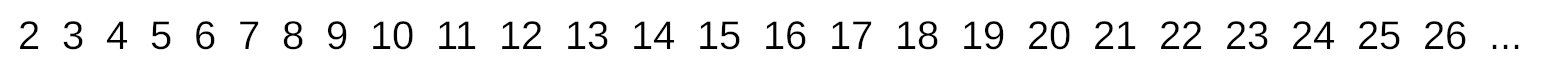
\includegraphics[width=\linewidth]{chapters/teorija-stevil/slike/reseto1}

Vemo, da je število $2$ praštevilo.
Večkratniki števila $2$ zato niso praštevila, ker so deljivi z $2$; torej jih
prečrtamo.

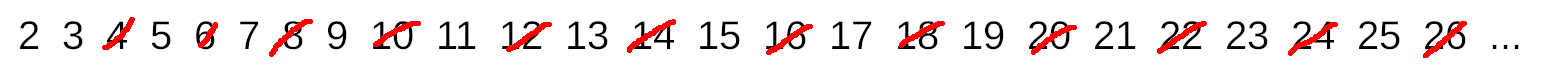
\includegraphics[width=\linewidth]{chapters/teorija-stevil/slike/reseto2}

Število $3$ je praštevilo, torej tudi večkratniki $3$ niso praštevila.

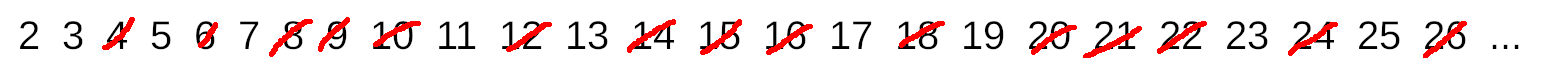
\includegraphics[width=\linewidth]{chapters/teorija-stevil/slike/reseto3}

Prišli so do števila $4$, ki je prečrtano, zato vemo, da ni praštevilo.
Ker je deljivo z $2$, smo vse večkratnike $4$ (ki so tudi večkratniki $2$), že
prečrtali, torej nam ni treba posebej črtati večkratnikov $4$.

Število $5$ je praštevilo (ker ni prečrtano), torej moremo prečrtati njegove
večkratnike.

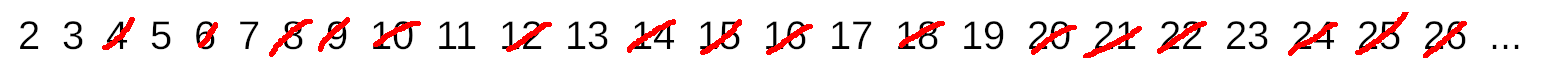
\includegraphics[width=\linewidth]{chapters/teorija-stevil/slike/reseto4}

Število $6$ je prečrtano, tako da ga preskočimo.

Postopek bi lahko nadaljevali, dokler ne pridemo do $26$ (oz.~do želene zgornje
meje), vendar nam ni treba.
Velja namreč naslednje; če je število $M$ produkt dveh števil, $M = A B$, potem
je vsaj eno od teh števil manjše od ali enako veliko kot $\sqrt{M}$.
Če bi bili obe števili večji kot $\sqrt{M}$, je njun produkt večji od $M$, to pa
ne mora veljati, ker je njun produkt ravno $M$.

V našem primeru smo torej lahko iskanje ustavili že pri $\sqrt{26}$, kar je
nekaj več kot $5$, zato moramo preveriti tudi $6$, več pa ne.

\begin{examples}
  Možna implementacija algoritma za iskanje praštevil je podana spodaj.
  Zapisana koda ohranja še dodatno informacijo; za vsako število si zapomnimo
  enega od njegovih praštevilskih deliteljev.
  %#insert python3 style.py < chapters/teorija-stevil/reseto.cpp
  Ta implementacija nam dovoljuje, da hitro poiščemo nekega delitelja poljubnega
  števila \verb+n+; preprosto pogledamo v \verb+reseto[n]+.
  Če najdemo \verb+0+, vemo, da je \verb+n+ praštevilo; sicer pa smo našli
  nekega delitelja.
\end{examples}

%#endblock
% LocalWords:  NSD
